\section{Empirical Results}
\label{results}
We experiment with both versions of our method (standard and online) on three kinds of benchmarks for distribution shifts, presented here in the order of visually low to high-level.
Our code is available at the project website.

\begin{figure*}
	\centering
	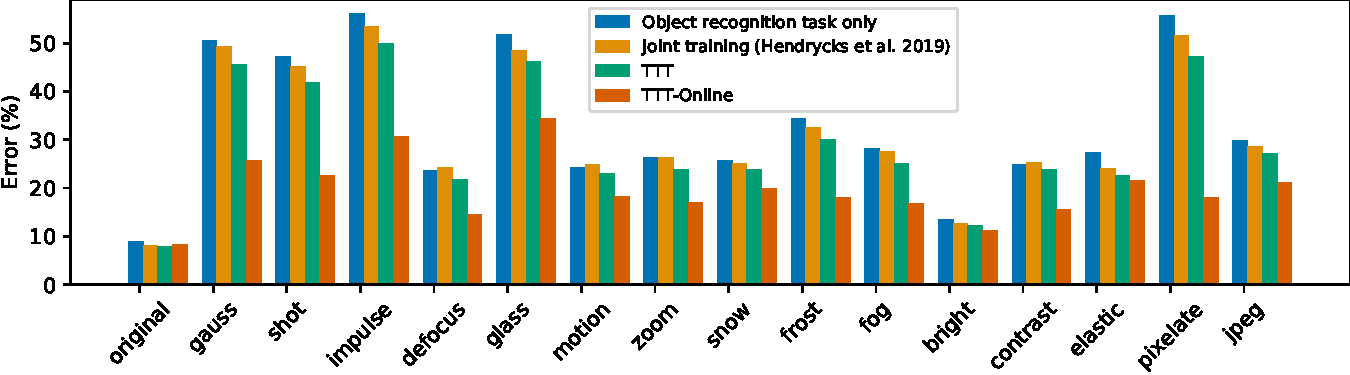
\includegraphics[width=1.0\textwidth]{plots/C10C_layer2_5_gn_expand_final}
	\caption{
	{\bf Test error (\%) on CIFAR-10-C with level 5 corruptions.} We compare our approaches, Test-Time Training (TTT) and its online version (TTT-Online), with two baselines: object recognition without self-supervision, and joint training with self-supervision but keeping the model fixed at test time. 
	TTT improves over the baselines and TTT-Online improves even further. 
	}
	\label{fig:cc}
\end{figure*}
\paragraph{Network details.}
Our architecture and hyper-parameters are consistent across all experiments.  We use ResNets \citep{he2016identity}, which are constructed differently for CIFAR-10 \citep{krizhevsky2009learning} (26-layer) and ImageNet \citep{ILSVRC15} (18-layer). The CIFAR-10 dataset contains 50K images for training, and 10K images for testing. The ImageNet contains 1.2M images for training and the 50K validation images are used as the test set. ResNets on CIFAR-10 have three groups, each containing convolutional layers with the same number of channels and size of feature maps; our splitting point is the end of the second group. ResNets on ImageNet have four groups;  our splitting point is the end of the third group. 

We use Group Normalization (GN) instead of Batch Normalization (BN) in our architecture, since BN has been shown to be ineffective when training with small batches, for which the estimated batch statistics are not accurate \citep{ioffe2015batch}. This technicality hurts Test-Time Training since each batch only contains (augmented) copies of a single image. Different from BN, GN is not dependent on batch size and achieves similar results on our baselines. We report results with BN in \Cref{results_additional} of the appendix for completeness. 
We directly compare our architecture to that of \citet{hendrycks2018using} in \autoref{reviewer_stuff}.

\begin{figure*}[t]
	\centering
	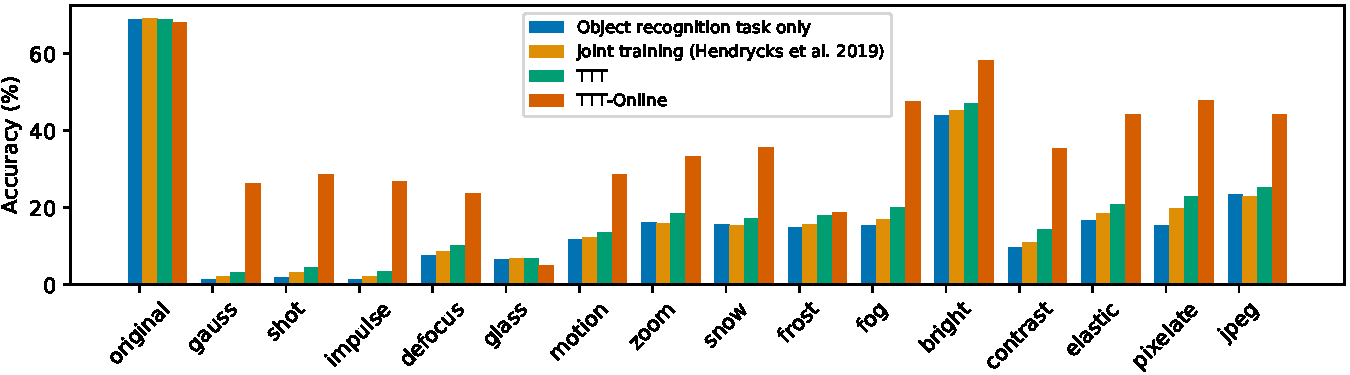
\includegraphics[width=1.0\textwidth]{plots/test_layer3_5_gn}
		\vspace{-2ex}
	\begin{subfigure}[b]{1.0\textwidth}
		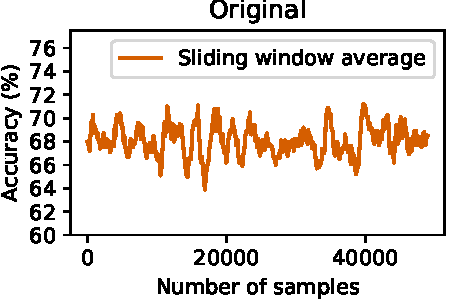
\includegraphics[width=0.325\textwidth]{plots/online_curves/original_5_avg}
		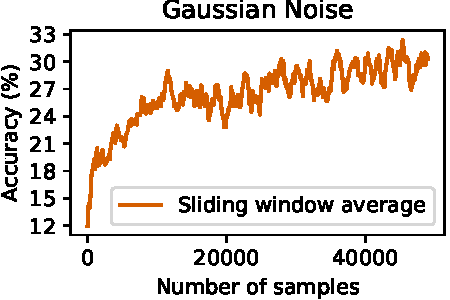
\includegraphics[width=0.325\textwidth]{plots/online_curves/gaussian_noise_5_avg}
		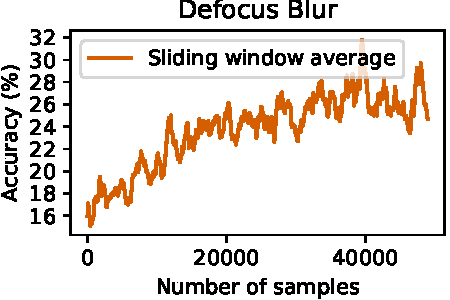
\includegraphics[width=0.325\textwidth]{plots/online_curves/defocus_blur_5_avg}
	\end{subfigure}
	\begin{subfigure}[b]{1.0\textwidth}
			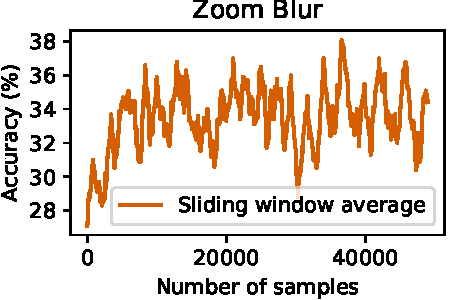
\includegraphics[width=0.325\textwidth]{plots/online_curves/zoom_blur_5_avg}
			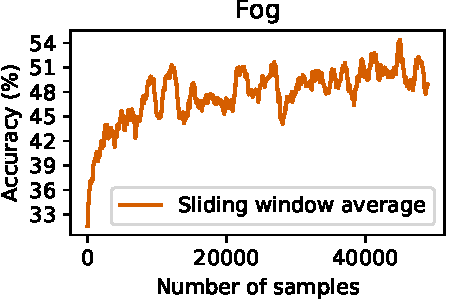
\includegraphics[width=0.325\textwidth]{plots/online_curves/fog_5_avg}
			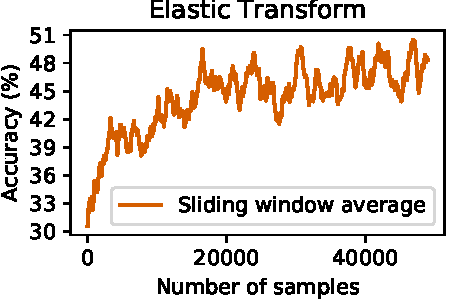
\includegraphics[width=0.325\textwidth]{plots/online_curves/elastic_transform_5_avg}
	\end{subfigure}
	\caption{
		{\bf Test accuracy (\%) on ImageNet-C with level 5 corruptions.} Upper panel: Our approaches, TTT and TTT-Online, show significant improvements in all corruption types over the two baselines. 
		Lower panel: We show the accuracy of TTT-Online as the average over a sliding window of 100 samples; TTT-Online generalizes better as more samples are evaluated (x-axis), without hurting on the original distribution. We use accuracy instead of error here because the baseline performance is very low for most corruptions.
	}
	\label{fig:cc_imagenet}
	\vspace{-1ex}
\end{figure*}
\paragraph{Optimization details.}
For joint training (\autoref{optimize_train}),
we use stochastic gradient descent with standard hyper-parameters as \citep{huang2016deep, he2016deep}.
For Test-Time Training (\autoref{optimize_test}), we use stochastic gradient descent with the learning rate set to that of the last epoch during training, which is 0.001 in all our experiments. We set weight decay and momentum to zero during Test-Time Training, inspired by practice in \citep{he2018rethinking, liu2018rethinking}. For the standard version of Test-Time Training, we take ten gradient steps, using batches independently generated by the same image.
For online version of Test-Time Training, we take only one gradient step given each new image. We use random crop and random horizontal flip for data augmentation. See \Cref{computational} of the appendix for computational aspects of our method.
In all the tables and figures, \emph{object recognition task only} refers to the plain ResNet model (using GN, unless otherwise specified);
\emph{joint training}
refers to the model jointly trained on both the main task and the self-supervised task, fixed at test time; this has been proposed as the method in \citet{hendrycks2019using};
\emph{Test-Time Training (TTT)}  refers to the standard version described \autoref{method};
and \emph{online Test-Time Training (TTT-Online)}  refers to the online version that does not discard $\vtheta(x_t)$ for $x_t$ arriving sequentially from the same distribution.
Performance for TTT-Online is calculated as the average over the entire test set; we always shuffle the test set before TTT-Online to avoid ordering artifacts.

\subsection{Object Recognition on Corrupted Images}
\label{results_cc}
\citet{hendrycks2019benchmarking} propose to benchmark robustness of object recognition with 15 types of corruptions
from four broad categories: noise, blur, weather and digital.  Each corruption type comes in five levels of severity, with level 5 the most severe (details and sample images in the appendix).
The corruptions are simulated to mimic real-world corruptions as much as possible on copies of the test set for both CIFAR-10 and ImageNet. The new test sets are named as CIFAR-10-C and ImageNet-C, respectively. 
In the proposed benchmark, training should be done on the original training set, and the diversity of corruption types should make it difficult for any methods to work well across the board if it relies too much on corruption specific knowledge. For online Test-Time Training, we take the entire test set as a stream of incoming images, and update and test on each image in an online manner as it arrives.

\paragraph{CIFAR-10-C.}
Our results on the level 5 corruptions (most severe) are shown in \autoref{fig:cc}.
The results on levels 1-4 are shown in
\Cref{results_additional} in appendix. 
Across all five levels and 15 corruption types, both standard and online versions of Test-Time Training improve over the object recognition task only baseline by a large margin. 
The standard version always improves over joint training, and the online version often improves significantly ($>$10\%) over joint training and never hurts by more than 0.2\%. 
Specifically, TTT-Online contributes $>$24\% on the three noise types and 38\% on pixelation. 
For a learning problem with the seemingly unstable setup that abuses a single image, this kind of consistency is rather surprising.

The baseline ResNet-26 with object recognition task only has error 8.9\% on the original test set of CIFAR-10. The joint training baseline actually improves performance on the original to 8.1\%. More surprisingly, unlike many other methods that trade off original performance for robustness, Test-Time Training further improves on the original test set by 0.2\% consistently over multiple independent trials. This suggests that our method does not choose between specificity and generality.

\newpage
Separate from our method, it is interesting to note that joint training consistently improves over the single-task baseline, as discovered by \citet{hendrycks2019using}.
\citet{hendrycks2019benchmarking} have also experimented with various other training methods on this benchmark, and point to Adversarial Logit Pairing (ALP) \citep{kannan2018adversarial} as the most effective approach. 
Results of this additional baseline on all levels of CIFAR-10-C are shown in the appendix, along with its implementation details. While surprisingly robust under some of the most severe corruptions (especially the three noise types), ALP incurs a much larger error (by a factor of two) on the original distribution and some corruptions (e.g. all levels of contrast and fog), and hurts performance significantly when the corruptions are not as severe (especially on levels 1-3); 
this kind of tradeoff is to be expected for methods based on adversarial training.

\begin{table*}[ht]
	\footnotesize
	\begin{center}
		{
			\setlength\tabcolsep{4.5pt}
			\renewcommand{\arraystretch}{1.5}
			\begin{tabular}{c|c|c|c|c|c|c|c|c|c|c|c|c|c|c|c|c}
				\hline
				& orig& gauss& shot& impul& defoc& glass& motn& zoom& snow& frost& fog& brit& contr& elast& pixel& jpeg\\
				\hline
				TTT-Online & \textbf{8.2}& \textbf{25.8}& \textbf{22.6}& 30.6& \textbf{14.6}& \textbf{34.4}& \textbf{18.3}& \textbf{17.1}& \textbf{20.0}& \textbf{18.0}& \textbf{16.9}& \textbf{11.2}& 15.6& \textbf{21.6}& \textbf{18.1}& \textbf{21.2}\\
				\hline
				UDA-SS & 9.0& 28.2& 26.5& \textbf{20.8}& 15.6& 43.7& 24.5& 23.8& 25.0& 24.9& 17.2& 12.7& \textbf{11.6}& 22.1& 20.3& 22.6\\
				\hline
			\end{tabular}
			\renewcommand{\arraystretch}{1}
		}
	\end{center}
	\caption{
		{\bf Test error (\%) on CIFAR-10-C with level 5 corruption.} Comparison between online Test-Time Training (TTT-Online) and unsupervised domain adaptation by self-supervision (UDA-SS)~\citep{sun2019uda} with access to the entire (unlabeled) test set during training. We highlight the lower error in bold. We have abbreviated the names of the corruptions, in order: original test set, Gaussian noise, shot noise, impulse noise, defocus blur, glass blue, motion blur, zoom blur, snow, frost, fog, brightness, contrast, elastic transformation, pixelation, and JPEG compression. 
		The reported numbers for TTT-Online are the same as in \autoref{fig:cc}.
		See complete table in \autoref{table:full_c10c}.
	}
\label{table:uda}
\end{table*} 
\begin{figure*}[ht]
	\centering
	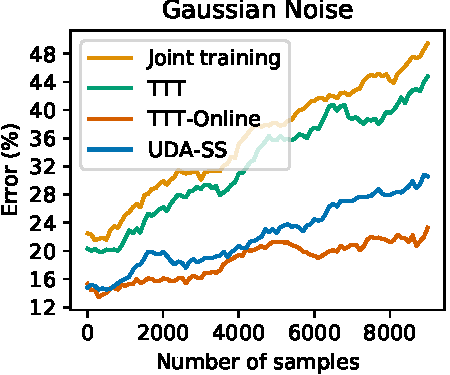
\includegraphics[width=0.33\textwidth]{plots/smooth/gaussian_noise_12345_avg.pdf}
	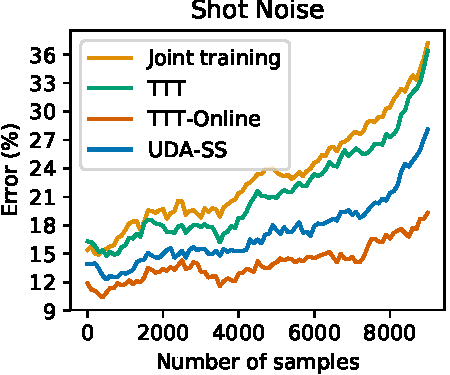
\includegraphics[width=0.33\textwidth]{plots/smooth/shot_noise_12345_avg.pdf}
	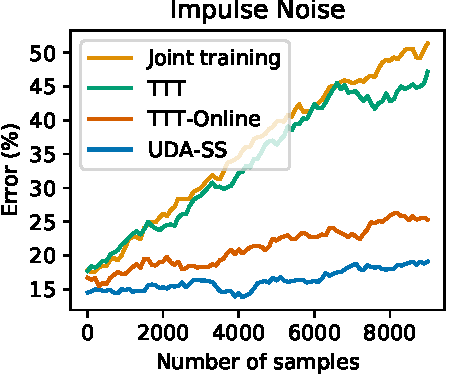
\includegraphics[width=0.33\textwidth]{plots/smooth/impulse_noise_12345_avg.pdf}
    
	\caption{
		{\bf Test error (\%) on CIFAR-10-C, for the three noise types, with gradually changing distribution.}
		The distribution shifts are created by increasing the standard deviation of each noise type from small to large, the further we go on the x-axis. As the samples get noisier, all methods suffer greater errors the more we evaluate into the test set, but online Test-Time Training (TTT-Online) achieves gentler slopes than joint training. For the first two noise types, TTT-Online also achieves better results over unsupervised domain adaptation by self-supervision (UDA-SS)~\citep{sun2019uda}.
	}
	\label{fig:smooth}
% 	\vspace{-2ex}
\end{figure*}

\paragraph{ImageNet-C.}
Our results on the level 5 corruptions (most severe) are shown in \autoref{fig:cc_imagenet}. We use accuracy instead of error for this dataset 
because the baseline performance is very low for most corruptions.
The general trend is roughly the same as on CIFAR-10-C. The standard version of TTT always improves over the baseline and joint training, while the online version only hurts on the original by 0.1\% over the baseline, but significantly improves (by a factor of more than three) on many of the corruption types.

In the lower panel of \autoref{fig:cc_imagenet}, we visualize how the accuracy (averaged over a sliding window) of the online version changes as more images are tested.
Due to space constraints, we show this plot on the original test set, as well as every third corruption type, following the same order as in the original paper. 
On the original test set, there is no visible trend in performance change after updating on the 50,000 samples.
With corruptions, accuracy has already risen significantly after 10,000 samples, but is still rising towards the end of the 50,000 samples, indicating room for additional improvements if more samples were available.
Without seeing a single label, TTT-Online behaves as if we were training on the test set from the appearance of the plots. 

\paragraph{Comparison with unsupervised domain adaptation.}
\autoref{table:uda} empirically compares online Test-Time Training (TTT-Online) with unsupervised domain adaptation through self-supervision (UDA-SS)~\citep{sun2019uda}, which is similar to our method in spirit but is designed for the setting of unsupervised domain adaptation (\Cref{related} provides a survey of other related work in this setting). 
Given labeled data from the training distribution and unlabeled data from the test distribution, UDA-SS hopes to find an invariant representation that extracts useful features for both distributions by learning to perform a self-supervised task, specifically rotation prediction, simultaneously on data from both. It then learns a labeling function on top of the invariant representation using the labeled data. In our experiments, the unlabeled data given to UDA-SS is the \emph{entire test set itself} without the labels.

Because TTT-Online can only learn from the unlabeled test samples that have already been evaluated on, it is given less information than UDA-SS at all times. In this sense, UDA-SS should be regarded as an oracle rather than a baseline.
Surprisingly, TTT-Online outperforms UDA-SS on 13 out of the 15 corruptions as well as the original distribution.
Our explanation is that UDA-SS has to find an invariant representation for both distributions, while TTT-Online only adapts the representation to be good for the current test distribution. That is, TTT-Online has the flexibility to  forget the training distribution representation, which is no longer relevant. This suggests that in our setting, forgetting is not harmful and perhaps should even be taken advantage of.

\paragraph{Gradually changing distribution shifts.}
In our previous experiments, we have been evaluating the online version under the assumption that the test inputs $x_t$ for $t=1...n$ are all sampled from the same test distribution $Q$, which can be different from the training distribution $P$. 
This assumption is indeed satisfied for i.i.d. samples from a shuffled test set.
But here we show that this assumption can in fact be relaxed to allow $x_t\sim Q_t$, where $Q_t$ is close to $Q_{t+1}$ (in the sense of distributional distance).
We call this the assumption of gradually changing distribution shifts. We perform experiments by simulating such distribution shifts on the three noise types of CIFAR-10-C. For each noise type, $x_t$ is corrupted with standard deviation $\sigma_t$, and $\sigma_1,...,\sigma_n$ interpolate between the standard deviation of level 1 and level 5. So $x_t$ is more severely corrupted as we evaluate further into the test set and $t$ grows larger.
As shown in \autoref{fig:smooth}, 
TTT-Online still improves upon joint training (and our standard version) with this relaxed assumption, and even upon UDA-SS for the first two noise types.

\begin{table*}[t!]
\begin{center}
{
\setlength\tabcolsep{4pt}
\begin{tabular}{c|ccccccc|c}
\toprule
Accuracy (\%)
		&Airplane	&Bird	&Car &Dog &Cat &Horse	&Ship  	&\textbf{Average}\\
\midrule
{\small Object recognition task only} & 67.9 & 35.8 & 42.6 & 14.7 & 52.0 & 42.0 & 66.7
&\textbf{41.4}\\
\midrule
{\small Joint training {\scriptsize \citep{hendrycks2019using}}} & 70.2 & 36.7 & 42.6 & 15.5 & 52.0 & 44.0 & 66.7
&\textbf{42.4}\\
\midrule
TTT (standard version) & 70.2 & 39.2 & 42.6 & 21.6 & 54.7 & 46.0 & 77.8
&\textbf{45.2}\\
\midrule 
TTT-Online & 70.2 & 39.2 & 42.6 & 22.4 & 54.7 & 46.0 & 77.8
&\textbf{45.4}\\
\bottomrule
\end{tabular}
}
\end{center}
\caption{
Class-wise and average classification accuracy (\%) on CIFAR classes in VID-Robust, adapted from \cite{shankar2019systematic}. Test-Time Training (TTT) and online Test-Time Training (TTT-Online) improve over the two baselines on average, and by a large margin on ``ship'' and ``dog'' classes where the rotation task is more meaningful than in classes like ``airplane'' (sample images in \autoref{vid_samples}). 
}
\label{table.cifar7}
\vspace{-1ex}
\end{table*} 


\subsection{Object Recognition on Video Frames}
\label{ivc}
The Robust ImageNet Video Classification (VID-Robust) dataset was developed by \citet{shankar2019systematic} from the ImageNet Video detection dataset \citep{ILSVRC15}, to demonstrate how deep models for object recognition trained on ImageNet (still images) fail to adapt well to video frames. The VID-Robust dataset contains 1109 sets of video frames in 30 classes; each set is a short video clip of frames that are similar to an anchor frame. Our results are reported on the anchor frames. To map the 1000 ImageNet classes to the 30 VID-Robust classes, we use the max-conversion function in \citet{shankar2019systematic}.
Without any modifications for videos, we apply our method to VID-Robust on top of the same ImageNet model as in the previous subsection. 
Our classification accuracy is reported in \autoref{vidtable}. 

In addition, we take the seven classes in VID-Robust that overlap with CIFAR-10, and re-scale those video frames to the size of CIFAR-10 images, as a new test set for the model trained on CIFAR-10 in the previous subsection. Again, we apply our method to this dataset without any modifications.
Our results are shown in \autoref{table.cifar7}, with a breakdown for each class. 
Noticing that Test-Time Training does not improve on the airplane class, we inspect some airplane samples (\autoref{vid_samples}), and observe black margins on two sides of most images, which provide a trivial hint for rotation prediction. 
In addition, given an image of airplanes in the sky, it is often impossible even for humans to tell if it is rotated.
This shows that our method requires the self-supervised task to be both well defined and non-trivial.

\subsection{CIFAR-10.1: Unknown Distribution Shifts}
\label{cifar10_new}
CIFAR-10.1 \citep{recht2018cifar} is a new test set of size 2000 modeled after CIFAR-10, with the exact same classes and image dimensionality, following the dataset creation process documented by the original CIFAR-10 paper as closely as possible.
The purpose is to investigate the distribution shifts present between the two test sets, and the effect on object recognition.
All models tested by the authors suffer a large performance drop on CIFAR-10.1 comparing to CIFAR-10,
even though there is no human noticeable difference, and both have the same human accuracy.
This demonstrates how insidious and ubiquitous distribution shifts are, even when researchers strive to minimize them.

\begin{table}
	\vspace{-1ex}
	\begin{center}{
			\begin{tabular}{c|c}  \toprule
				Method 									& Accuracy (\%) \\	\midrule
				{\small Object recognition task only} 								& 62.7\\  \midrule
				{\small Joint training {\scriptsize \citep{hendrycks2019using}}}						& 63.5\\  \midrule
				TTT	(standard version)	& 63.8\\  \midrule
				TTT-Online		& 64.3\\  \bottomrule
			\end{tabular}
			\caption{Test accuracy (\%) on VID-Robust dataset~\cite{shankar2019systematic}. 
			TTT and TTT-Online improve over the baselines.
			}\label{vidtable}
	}\end{center}
\end{table} 

\begin{table}
\begin{center}{
\begin{tabular}{c|c}  \toprule
Method 									& Error (\%) \\	\midrule
{\small Object recognition task only} 								
& 17.4\\  \midrule
{\small Joint training {\scriptsize \citep{hendrycks2019using}}}						
& 16.7\\  \midrule
TTT	(standard version)		& 15.9\\  \bottomrule
\end{tabular}
\caption{Test error (\%) on CIFAR-10.1~\cite{recht2018cifar}. TTT is the first method to improve the performance of an existing model on this new test set.}
\label{cifar10_new_table}
}\end{center}
\vspace{-3ex}
\end{table}


The distribution shifts from CIFAR-10 to CIFAR-10.1 pose an extremely difficult problem, and no prior work has been able to improve the performance of an existing model on this new test set, 
probably because:
1) researchers cannot even identify the distribution shifts, let alone describe them mathematically; 
2) the samples in CIFAR-10.1 are only revealed at test time; and even if they were revealed during training, the distribution shifts are too subtle, and the sample size is too small, for domain adaptation~\citep{recht2018cifar}.

On the original CIFAR-10 test set, the baseline with only object recognition has error 8.9\%,
and with joint training has 8.1\%;
comparing to the first two rows of \autoref{cifar10_new_table}, 
both suffer the typical performance drop (by a factor of two). 
TTT yields an improvement of 0.8\%
(relative improvement of 4.8\%) over joint training.
We recognize that this improvement is small relative to the performance drop, but see it as an encouraging first step for this very difficult problem.
